\newpage
\section{CUnit tests and simulation of the system}
In order to check the behaviour of the system a sequence of tests have been executed on the \textit{ESTA\_JSON\_lib} functions, that is used to convert the incoming JSON string from the module \textit{Room}.

\subsection{Variables tests}
For each variable present in the JSON message a boundary test is exeuted.
\newline
\begin{center}
	\begin{tabular}{|| c | c | c | c | c | c | c | c | c | c | c||} 
		\hline
		Variable				& 	Min 	& Max 	& 1\degree	& 2\degree & 3\degree	& 4\degree & 5\degree	& 6\degree & 7\degree\\ 
		\hline
		\textbf{Id}				&	1 		& 2		& 0 	& 1 	& 2 	& 3 	& / 	& / 	& / \\ 
		\hline
		\textbf{Eco}			&	0 		& 1		& -1  	& 0 	& 1 	& 2 	& / 	& /		& / \\ 
		\hline
		\textbf{Temperature}	&	15.0 	& 30.0	& 14.99 & 15.0 	& 15.01 & 29.99	& 30.00 & 30.01 & 22.5 \\ 
		\hline
		\textbf{Humidity}		&	0.0		& 100.0	& -0.01	& 0.0 	& 0.01 	& 99.99 & 100.00 & 100.01 & 50.00 \\ 
		\hline
		\textbf{Valve}			&	0		& 100 	& -1 	& 0 	& 1 	& 99 	& 100 	& 101 	& 50 \\ 
		\hline
	\end{tabular}
	\captionof{table}{Variables tests \label{tab:VariablesTests}}
\end{center}

\subsection{JSON Compliance  tests}
In order to check the \textit{JSON compliance code checker} the following tests are applied modifying a correct message.
\begin{center}
	\begin{tabular}{||c | c ||} 
		\hline
		Number			& 	Description \\ 
		\hline
		\textbf{1}		&	Missing odd number of \textit{\{}\\ 
		\hline
		\textbf{2}		&	Missing odd number of \textit{"}\\ 
		\hline
		\textbf{3}		&	Missing odd number of \textit{[}\\ 
		\hline
		\textbf{4}		&	Check field name \textit{Id} \\ 
		\hline
		\textbf{5}		&	Check field name \textit{Eco} \\ 
		\hline
		\textbf{6}		&	Check field name \textit{Nm} \\ 
		\hline
		\textbf{7}		&	Check field name \textit{Val} \\ 
		\hline
		\textbf{8}		&	Check field name \textit{Fmt} \\ 
		\hline
		\textbf{9}		&	Check field name \textit{Tmp} \\ 
		\hline
		\textbf{10}		&	Check field name \textit{Hum} \\ 
		\hline
		\textbf{11}		&	Check field name \textit{Vlv} \\ 
		\hline
		\textbf{12}		&	Check Temperature format value \textit{C} \\ 
		\hline
		\textbf{13}		&	Check Humidity format value \textit{\%} \\ 
		\hline
		\textbf{14}		&	Check Valve format value \textit{\%} \\ 
		\hline
	\end{tabular}
	\captionof{table}{JSON compliance tests \label{tab:JSONComplianceTests}}
\end{center}

In the following picture \ref{fig:CUnit_result} is reported the result of the tests executed using the framework \textit{CUnit} Version 2.1.3.
\begin{figure}[H]
	\centering
	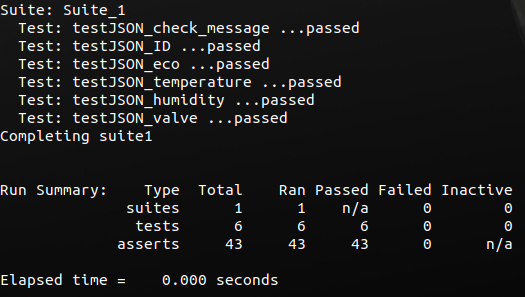
\includegraphics[width=8cm,keepaspectratio]{img/CUnit_result}
	\caption{CUnit results}
	\label{fig:CUnit_result}
\end{figure}


\subsection{Network noise tests}
In order to check the correctness behaviour of the \textit{Central Unit} module a python script that simulates the rooms has been created and used to test the module simulating two different rooms.
The \textbf{Room simulator} creates the correct JSON string and send it, in order to simulate the \textbf{noise} of the network this cases have been considered:
\begin{center}
	\begin{tabular}{||c | c | c ||} 
		\hline
		Number			& 	Description & Probability\\ 
		\hline
		\textbf{1}		&	Message lost, the response message is discarded & 0.1 \\ 
		\hline
		\textbf{2}		&	Message corrupted, 3 random characters are replaced with \textit{?} & 0.1\\ 
		\hline
	\end{tabular}
	\captionof{table}{Network noise tests \label{tab:NetworkNoiseTests}}
\end{center}
\begin{figure}[H]
	\centering
	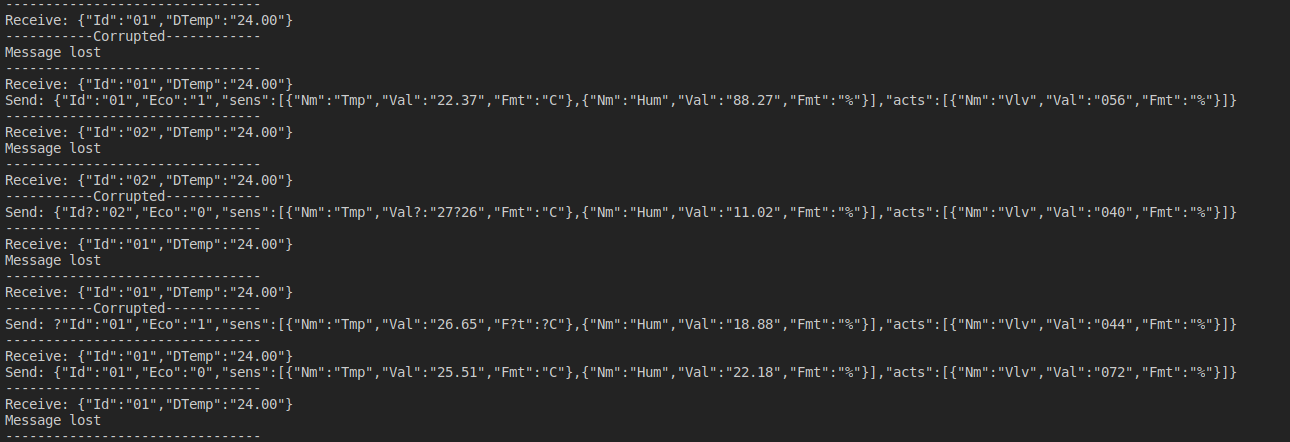
\includegraphics[width=12cm,keepaspectratio]{img/room_simulator}
	\caption{Room simulator}
	\label{fig:roomsimulator}
\end{figure}